\documentclass[11pt,a4paper]{book}
\usepackage[utf8]{inputenc}
\usepackage[spanish]{babel}
\usepackage{amsmath}
\usepackage{amsfonts}
\usepackage{amssymb}
\usepackage{graphicx} % figuras
\usepackage{subfigure} % subfiguras
\usepackage{enumerate} % enumerados
\author{Nombre y apellidos}
\usepackage{fancyhdr} 
\usepackage[margin=3cm]{geometry}

% encabezados
\lhead[\leftmark]{}
\chead[]{}
\rhead[]{\rightmark}
\renewcommand{\headrulewidth}{0.5pt}

% pie de pagina
\lfoot[\thepage]{Universidad Politécnica de Madrid}
\cfoot[]{}
\rfoot[Nombre y apellido Matricula]{\thepage}
\renewcommand{\footrulewidth}{0.5pt}

% primera pagina de un capitulo
\fancypagestyle{plain}{
\fancyhead[L]{}
\fancyhead[C]{}
\fancyhead[R]{}
\fancyfoot[L]{}
\fancyfoot[C]{}
\fancyfoot[R]{\thepage}
\renewcommand{\headrulewidth}{0pt}
\renewcommand{\footrulewidth}{0pt}
}

\pagestyle{fancy}

\begin{document}

\chapter{Estado del arte}

%\section{}	\label{sec:robots_usar}

%\begin{figure}[htb] \label{fig:pers_robs_USAR}
%\centering
%\subfigure[]{\includegraphics[width=50mm]{../imagenes/2_estado_del_arte/USAR.jpg}}
%\subfigure[]{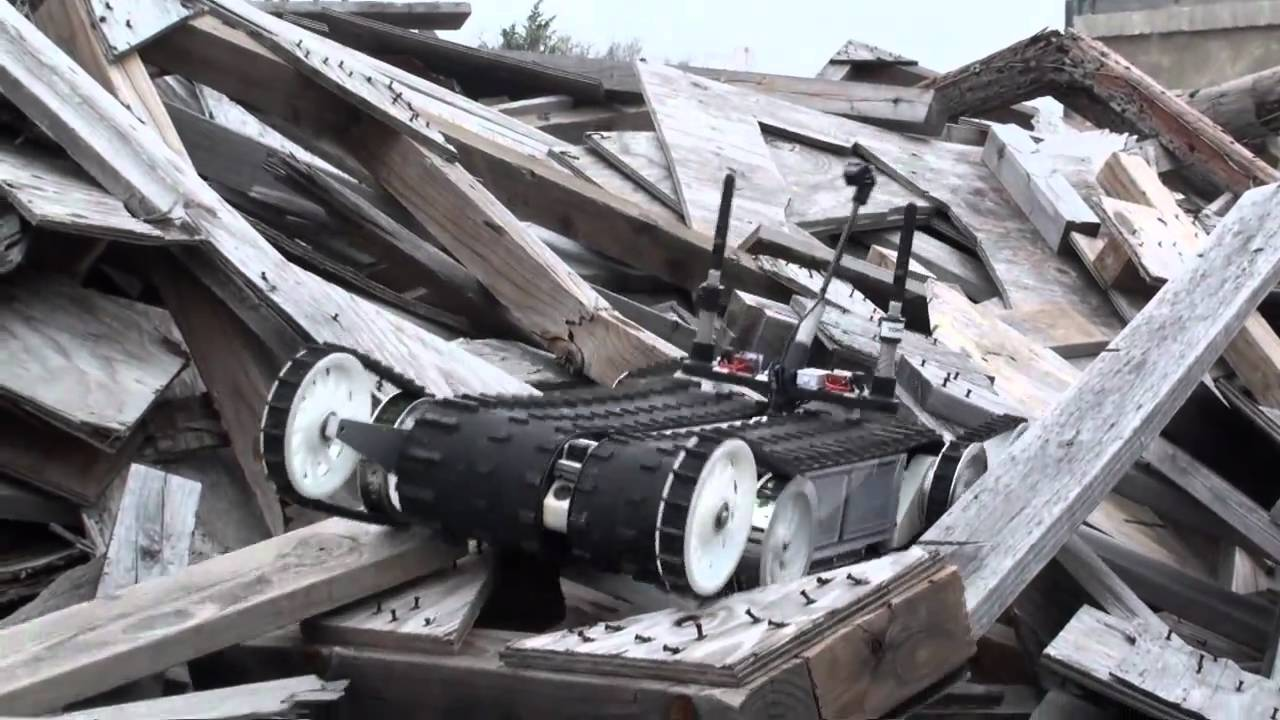
\includegraphics[width=50mm]{../imagenes/2_estado_del_arte/robot_rescate.jpg}}
%\caption{Robots y personal de busqueda y rescate}
%\end{figure}

% Estilo bibiolgrafia	
%\bibliographystyle{acm}
% Archivo bibliografia
%\bibliography{../DB_bibliografia/bib_tfg_raul_cebolla_13069}

\end{document}
